% Provenance (never printed): cycle 3 / 6e "La planete Terre, l'environnement
% et l'action humaine" (the Earth in the Solar System; conditions for life);
% see sources/book1/PROVENANCE.md. Book 1, grade 6, chapter 1.
\chapter{الأرض، كوكب من المجموعة الشمسية}\label{ch:g6:earth-a-planet}

أُرسلت ثلاثة مسابير آلية إلى الفضاء. ويرسل كل منها بدوره صورة إلى
الأرض، كأنها بطاقة بريدية. الأولى تأتي من الزهرة: كرة شاحبة
ملفوفة \omterm{def:g4:clouds-rain-snow:cloud}{بسحب} كثيفة، حرارتها تكفي لصهر الرصاص، وهواؤها
يضغط على الأرض بثقل ساحق. والثانية تأتي من المريخ:
\omterm{def:g5:weather-and-climate:desert}{صحراء} حمراء باردة مغبرة تحت سماء رقيقة. أما المسبار الثالث فقد أدار
آلة تصويره نحو موطنه: كرة زرقاء وبيضاء، فيها محيطات \omterm{def:g4:clouds-rain-snow:cloud}{وسحب}
وجليد. ثلاثة كواكب، جيران حول الشمس نفسها. فلماذا كان واحد منها
فقط أزرق؟
% ledger: nasa:venus-clouds, nasa:mars-water

\begin{omfigure}
\begin{minipage}[t]{0.31\linewidth}\centering
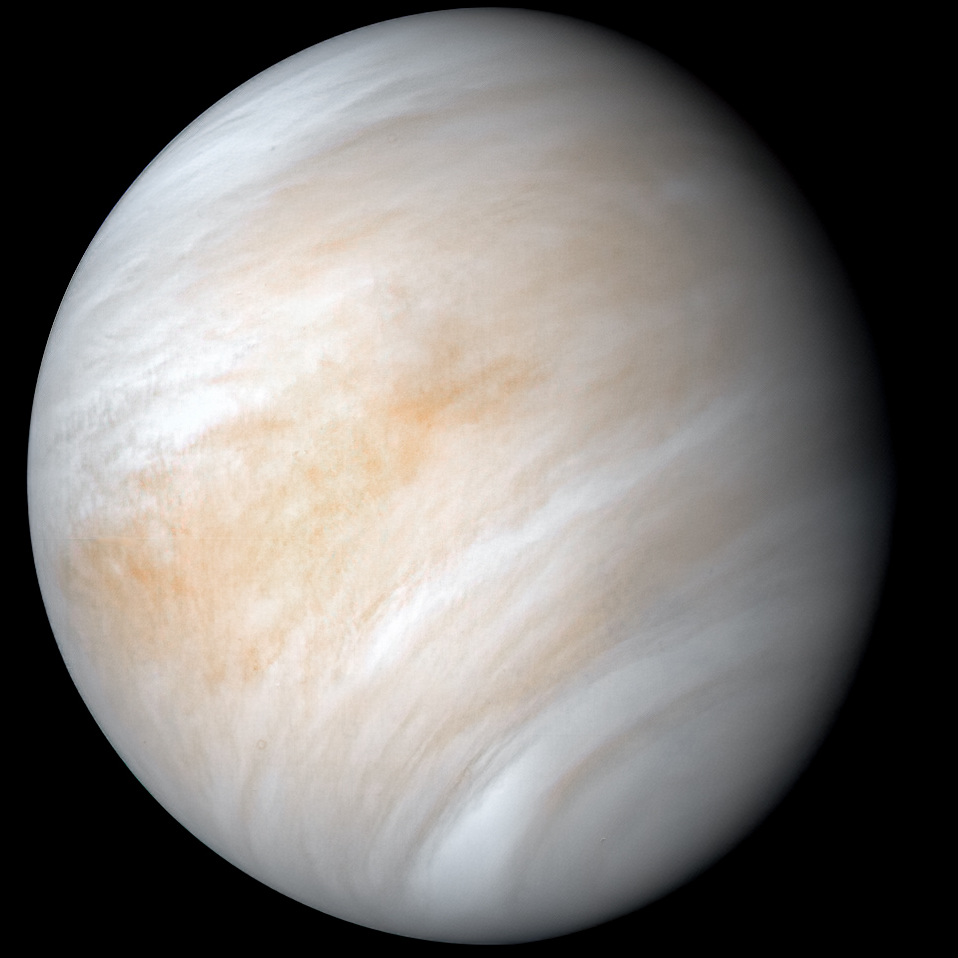
\includegraphics[width=\linewidth]{images/book1/g6-venus-mariner10.jpg}\\[2pt]
{\small الزهرة}
\end{minipage}\hfill
\begin{minipage}[t]{0.31\linewidth}\centering
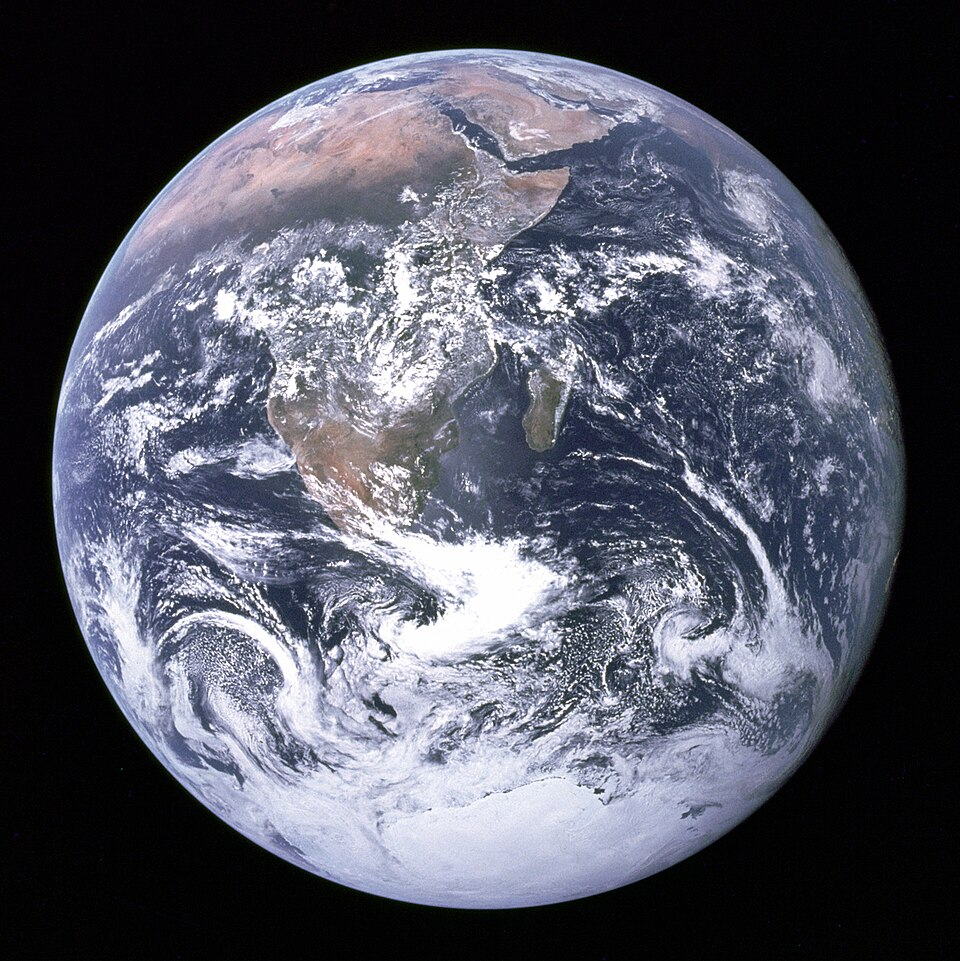
\includegraphics[width=\linewidth]{images/book1/g6-earth-apollo17.jpg}\\[2pt]
{\small الأرض}
\end{minipage}\hfill
\begin{minipage}[t]{0.31\linewidth}\centering
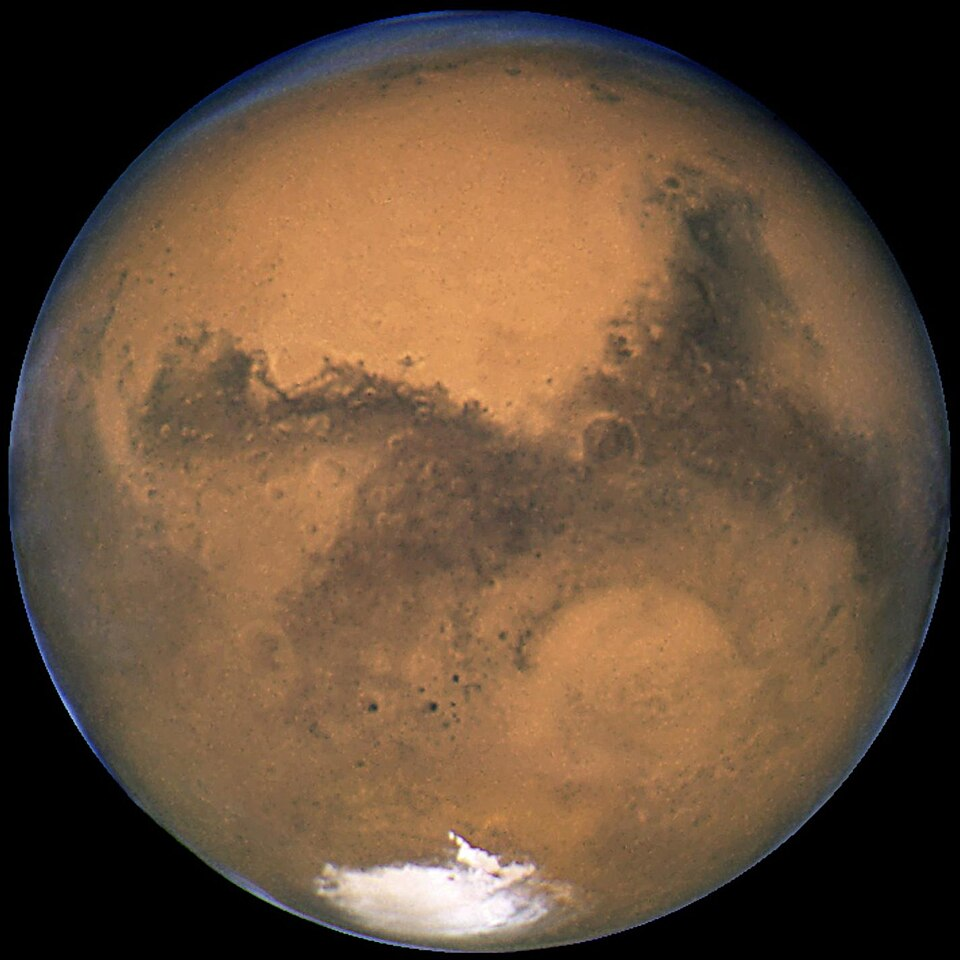
\includegraphics[width=\linewidth]{images/book1/g6-mars-hubble.jpg}\\[2pt]
{\small المريخ}
\end{minipage}

\medskip
{\small ثلاث بطاقات بريدية من الفضاء. الزهرة، كما صورها المسبار مارينر~10
عام 1974: لا نرى إلا أعلى سحبها. والأرض، كما صورها
طاقم أبولو~17 في طريقهم إلى القمر عام 1972: إفريقيا وشبه الجزيرة العربية
وجليد القارة القطبية الجنوبية تحت \omterm{def:g4:clouds-rain-snow:cloud}{سحب} بيضاء. والمريخ، كما صوره
مقراب هابل الفضائي عام 2003، وعلى قطبه قلنسوة بيضاء من الجليد.
(الصور: NASA/JPL-Caltech؛ NASA؛ NASA وESA وفريق تراث هابل.)}
% ledger: nasa:venus-mariner10, nasa:apollo17-earth, hubble:mars-2003
\end{omfigure}

\begin{recall}
بيّنت كتب الفيزياء أن الشمس نجم، كرة هائلة من الغاز الحار
تضيء بنفسها، وأن الكوكب جسم كبير مستدير يدور
حول نجم ولا يضيء بنفسه: نراه لأنه يعكس
ضوء نجمه. والشمس وكل ما يدور حولها تشكل
المجموعة الشمسية. وكل كوكب يسير حول الشمس على مسار يسمى
مداره، ويدور حول نفسه حول محور. والهواء من حولنا يضغط
على كل ما يلمسه: ذلك هو ضغط الهواء. وكثافة مادة ما
تخبرنا كم يزن حجم معيّن منها: فالسنتيمتر المكعب من الماء
يزن 1~غرامًا، فكثافته 1~غرام لكل سنتيمتر مكعب؛ والمادة
الأكثف من الماء تغطس فيه، والمادة الأقل كثافة تطفو. وأخيرًا، نحو سبعة أعشار
سطح الأرض يغطيها \omterm{def:g2:water-on-earth:ocean}{المحيط}
(\cref{ch:g2:water-on-earth}).
\end{recall}

\section{ثمانية كواكب حول الشمس}

ثمانية كواكب تسير حول الشمس. وهي بالترتيب، من الأقرب إلى
الأبعد: عطارد، والزهرة، والأرض، والمريخ، والمشتري، وزحل،
وأورانوس، ونبتون. ويمكن أن تساعدك جملة على تذكر الترتيب: \emph{عُمَر
زارَ أخاه مساءً مع زوجته، أكلوا نبقًا} (عطارد، الزهرة، الأرض، المريخ،
المشتري، زحل، أورانوس، نبتون).

الرسم أدناه يبين الكواكب الثمانية جنبًا إلى جنب، مرسومة بمقياس
الرسم نفسه: فإذا كان كوكب أعرض من آخر مرتين، كانت دائرته أعرض
مرتين أيضًا.

\begin{omfigure}
\pgfplotstableread{figdata/out/grade-6-planets-sizes.dat}\gsixsizes
\begin{tikzpicture}
  \draw[black!40] (-0.2,0) -- (13.8,0);
  \pgfplotstablegetrowsof{\gsixsizes}
  \pgfmathtruncatemacro{\gsixlast}{\pgfplotsretval-1}
  \foreach \i in {0,...,\gsixlast}{
    \pgfplotstablegetelem{\i}{x_cm}\of\gsixsizes \let\gx\pgfplotsretval
    \pgfplotstablegetelem{\i}{d_cm}\of\gsixsizes \let\gd\pgfplotsretval
    \def\gn{\ifcase\i عطارد\or الزهرة\or الأرض\or المريخ\or المشتري\or زحل\or أورانوس\or نبتون\fi}
    \pgfplotstablegetelem{\i}{d_km}\of\gsixsizes \let\gk\pgfplotsretval
    \pgfmathsetmacro{\gr}{\gd/2}
    \ifnum\i<4
      \fill[brown!70!black, draw=black!60, line width=0.3pt] (\gx,\gr) circle (\gr);
    \else
      \fill[orange!35, draw=black!60, line width=0.3pt] (\gx,\gr) circle (\gr);
    \fi
    \node[font=\scriptsize, rotate=40, anchor=north east, inner sep=1pt]
      at (\gx+0.08,-0.08) {\gn};
  }
  \node[font=\scriptsize, align=left, anchor=north west] at (-0.2,4.15)
    {\foreignlanguage{arabic}{\tikz\fill[brown!70!black, draw=black!60] (0,0) circle (2.2pt); كواكب صخرية}\\
     \foreignlanguage{arabic}{\tikz\fill[orange!35, draw=black!60] (0,0) circle (2.2pt); كواكب عملاقة}};
  \draw[|-|, black!70] (0,2.2) -- (1,2.2)
    node[midway, above, font=\scriptsize] {35\,000 km};
\end{tikzpicture}

{\small الكواكب الثمانية مرسومة بمقياس الرسم (الأقطار من صحيفة بيانات
الكواكب لدى NASA). أما المسافات بينها فليست بمقياس الرسم: فهي
أكبر بكثير من أن تتسع لها أي صفحة.}
% ledger: planet:Mercury.diameter, planet:Venus.diameter, planet:Earth.diameter, planet:Mars.diameter, planet:Jupiter.diameter, planet:Saturn.diameter, planet:Uranus.diameter, planet:Neptune.diameter (figdata/grade-6/planets.py, part sizes)
\end{omfigure}

الكواكب الأربعة الأقرب إلى الشمس صغيرة. والأربعة التالية عمالقة:
فالمشتري أعرض من الأرض بنحو 11 مرة. والشمس؟ لو رُسمت \omterm{def:g2:drawing-to-map:scale}{بمقياس
رسم} الكواكب أعلاه نفسه، لكانت قرصًا قطره نحو 40~سنتيمترًا
--- أعرض من هذه الصفحة.
% ledger: planet:Jupiter.diameter, planet:Earth.diameter, sun:R (planets.py: sun_cm = 39.9 cm)

الحجم ليس الفرق الوحيد. فالجدول أدناه يعطي، لكل كوكب،
قطره، وكثافته (بالغرامات لكل سنتيمتر مكعب)، وبعده
عن الشمس.

\begin{center}
\small
\begin{tabular}{lrrrr}
\hline
الكوكب & القطر (km) & الكثافة (\babelsublr{g/cm$^3$}) & البعد عن الشمس (مليون km)\\
\hline
عطارد & 4\,879 & 5.4 & 58\\
الزهرة & 12\,104 & 5.2 & 108\\
الأرض & 12\,756 & 5.5 & 150\\
المريخ & 6\,792 & 3.9 & 228\\
\hline
المشتري & 142\,984 & 1.3 & 779\\
زحل & 120\,536 & 0.7 & 1\,432\\
أورانوس & 51\,118 & 1.3 & 2\,867\\
نبتون & 49\,528 & 1.6 & 4\,515\\
\hline
\end{tabular}
% ledger: planet:Mercury.diameter, planet:Venus.diameter, planet:Earth.diameter, planet:Mars.diameter, planet:Jupiter.diameter, planet:Saturn.diameter, planet:Uranus.diameter, planet:Neptune.diameter, planet:Mercury.density, planet:Venus.density, planet:Earth.density, planet:Mars.density, planet:Jupiter.density, planet:Saturn.density, planet:Uranus.density, planet:Neptune.density, planet:Mercury.dist, planet:Venus.dist, planet:Earth.dist, planet:Mars.dist, planet:Jupiter.dist, planet:Saturn.dist, planet:Uranus.dist, planet:Neptune.dist (figdata/grade-6/planets.py, main table)
\end{center}

الكثافات تقسم الكواكب إلى فصيلتين، لا شيء بينهما:
فالأربعة الأولى كثيفة، أكثر من 3.9~غرام لكل سنتيمتر مكعب، مثل
\omterm{def:g3:stones-pebbles-sand:rock}{الصخر} والفلز؛ والأربعة الأخيرة خفيفة، أقل من 1.7~غرام لكل سنتيمتر
مكعب.

\begin{definition}[الكواكب الصخرية والكواكب العملاقة]\label{def:g6:earth-a-planet:planet-types}
\emph{الكوكب الصخري}\index{كوكب صخري} كوكب صغير كثيف مصنوع من
\omterm{def:g3:stones-pebbles-sand:rock}{الصخر} والفلز، له سطح صلب يستطيع مسبار أن يهبط عليه: عطارد،
والزهرة، والأرض، والمريخ. و\emph{الكوكب العملاق}\index{كوكب عملاق}
كوكب كبير جدًا قليل الكثافة، مصنوع في معظمه من الغازات والسوائل، ولا
سطح صلبًا له يُهبط عليه: المشتري، وزحل، وأورانوس، ونبتون.
% ledger: nasa:planet-families
\end{definition}

\begin{omfigure}
\begin{minipage}[c]{0.6\linewidth}\centering
\begin{tikzpicture}
  \begin{axis}[ybar, bar width=11pt, width=\linewidth, height=5.4cm,
      ymin=0, ymax=6.2, xmin=-0.6, xmax=7.6,
      xtick={0,...,7}, xticklabels={عطارد,الزهرة,الأرض,المريخ,المشتري,زحل,أورانوس,نبتون},
      xticklabel style={rotate=40, anchor=north east, font=\scriptsize},
      ytick={0,1,...,6}, ylabel={\foreignlanguage{arabic}{الكثافة \babelsublr{(g/cm$^3$)}}},
      tick label style={font=\scriptsize}, label style={font=\scriptsize},
      axis x line*=bottom, axis y line*=left]
    \addplot[fill=brown!70!black, draw=black!60, bar shift=0pt, restrict x to domain=0:3]
      table[x=idx, y=density_gcm3] {figdata/out/grade-6-planets-density.dat};
    \addplot[fill=orange!35, draw=black!60, bar shift=0pt, restrict x to domain=4:7]
      table[x=idx, y=density_gcm3] {figdata/out/grade-6-planets-density.dat};
    \draw[blue!60!black, densely dashed] (axis cs:-0.6,1) -- (axis cs:7.6,1);
    \node[font=\scriptsize, blue!60!black, anchor=south, inner sep=1pt]
      at (axis cs:5,1) {الماء};
  \end{axis}
\end{tikzpicture}
\end{minipage}\hfill
\begin{minipage}[c]{0.36\linewidth}\centering
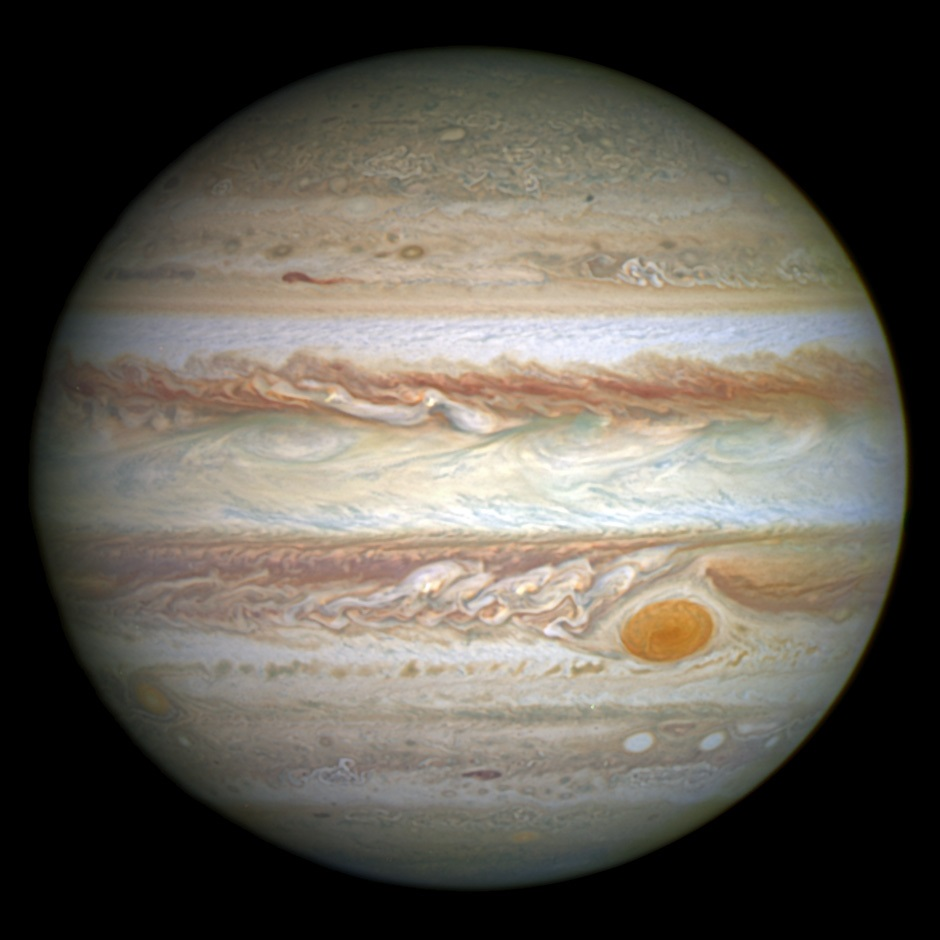
\includegraphics[width=0.9\linewidth]{images/book1/g6-jupiter-hubble.jpg}\\[2pt]
{\small المشتري، كما صوره مقراب هابل الفضائي عام 2014.
(الصورة: NASA، وESA، وأ.~سايمون.)}
% ledger: hubble:jupiter-2014
\end{minipage}

\smallskip
{\small إلى اليمين: كثافة الكواكب الثمانية؛ والخط المتقطع هو
كثافة الماء. إلى اليسار: ما نراه من \omterm{def:g6:earth-a-planet:planet-types}{كوكب عملاق} هو أعلى
سحبه.}
% ledger: planet:Mercury.density, planet:Venus.density, planet:Earth.density, planet:Mars.density, planet:Jupiter.density, planet:Saturn.density, planet:Uranus.density, planet:Neptune.density (figdata/grade-6/planets.py, part density)
\end{omfigure}

صورة المشتري تبين أشرطة من \omterm{def:g4:clouds-rain-snow:cloud}{السحب}، فاتحة وداكنة، وشكلًا بيضويًا
أحمر: البقعة الحمراء العظيمة، \omterm{def:g5:natural-hazards:storm}{عاصفة} عملاقة أكبر من الأرض كلها،
تهب منذ مئات السنين. وتحت \omterm{def:g4:clouds-rain-snow:cloud}{السحب} لا توجد أرض:
بل غازات فقط، معظمها الهيدروجين والهيليوم، تزداد كثافة كلما
تعمقنا.
% ledger: nasa:jupiter-gas

\begin{remark}[كوكب أخف من الماء]\label{rem:g6:earth-a-planet:saturn}
زحل هو الكوكب الوحيد الذي كثافته أقل من كثافة الماء: نحو
0.7~غرام لكل سنتيمتر مكعب. فلو وُجد حوض استحمام كبير بما يكفي
ليسعه، لطفا زحل!
% ledger: nasa:saturn-float, planet:Saturn.density
\end{remark}

\section{كم تتباعد الكواكب؟}

الكواكب لا تختلف كثيرًا في الحجم فحسب؛ بل هي أيضًا بعيدة جدًا
بعضها عن بعض. فالأرض على بعد نحو 150~مليون كيلومتر من الشمس.
ونبتون، أبعد الكواكب، أبعد منها 30~مرة: نحو 4500~مليون
كيلومتر. والرسم أدناه يضع الكواكب الثمانية على خط واحد، على
أبعادها عن الشمس، بمقياس الرسم.
% ledger: planet:Earth.dist, planet:Neptune.dist

\begin{omfigure}
\begin{tikzpicture}
  % whole system
  \draw[thick, gray] (0,0) -- (13.6,0);
  \fill[orange!80!yellow] (0,0) circle (3pt);
  \node[font=\scriptsize, above=3pt] at (0,0) {الشمس};
  \foreach \n/\x/\lab in {Mercury/0.174/, Venus/0.326/, Earth/0.451/, Mars/0.687/,
                          Jupiter/2.345/المشتري, Saturn/4.313/زحل, Uranus/8.636/أورانوس, Neptune/13.6/نبتون} {
    \fill (\x,0) circle (1.4pt);
    \node[font=\scriptsize, above=3pt] at (\x,0) {\lab};
  }
  \draw[decorate, decoration={brace, amplitude=3pt, mirror}] (0.1,-0.25) -- (0.75,-0.25)
    node[midway, below=3pt, font=\scriptsize, align=center] {الكواكب\\ الصخرية الأربعة};
  \draw[<->, thin, gray!70!black] (0,0.62) -- (13.6,0.62) node[midway, above, font=\scriptsize, black] {\foreignlanguage{arabic}{من الشمس إلى نبتون: نحو \babelsublr{4500} مليون كيلومتر}};
  % the inner system, ten times larger
  \begin{scope}[yshift=-2.3cm]
    \draw[thick, gray] (0,0) -- (7.6,0);
    \fill[orange!80!yellow] (0,0) circle (3pt);
    \node[font=\scriptsize, above=3pt] at (0,0) {الشمس};
    \foreach \n/\x in {عطارد/1.744, الزهرة/3.259, الأرض/4.506, المريخ/6.868} {
      \fill (\x,0) circle (1.4pt);
      \node[font=\scriptsize, below=3pt] at (\x,0) {\n};
    }
    \node[font=\scriptsize, anchor=west, align=left] at (8.0,0) {الخط نفسه، أطول عشر مرات\\ للكواكب الصخرية};
  \end{scope}
  \draw[dashed, gray] (0.75,-0.05) -- (7.6,-2.15);
\end{tikzpicture}

{\small أبعاد الكواكب عن الشمس، بمقياس الرسم. في الأعلى: المجموعة
الشمسية كلها، من الشمس إلى نبتون. في الأسفل: \omterm{def:g6:earth-a-planet:planet-types}{الكواكب الصخرية} الأربعة،
مكبّرة عشر مرات. أما أحجام النقاط فليست بمقياس الرسم.}
% ledger: planet:Mercury.dist, planet:Venus.dist, planet:Earth.dist, planet:Mars.dist, planet:Jupiter.dist, planet:Saturn.dist, planet:Uranus.dist, planet:Neptune.dist (figdata/grade-6/planets.py, part dist)
\end{omfigure}

\omterm{def:g6:earth-a-planet:planet-types}{الكواكب الصخرية} الأربعة كلها قريبة من الشمس؛ \omterm{def:g6:earth-a-planet:planet-types}{والكواكب العملاقة} الأربعة
بعيدة، بينها فجوات هائلة. والفجوة بين المريخ والمشتري وحدها، نحو 550~مليون كيلومتر، أكبر من ضعف المسافة بين الشمس والمريخ.
% ledger: planet:Mars.dist, planet:Jupiter.dist

من الصعب أن نرسم الأحجام والمسافات بمقياس رسم واحد: فالكواكب
تصير نقاطًا لا تُرى. و\emph{النموذج المصغر} يساعد على تخيلهما معًا.

\begin{method}[بناء نموذج مصغر للمجموعة الشمسية]\label{met:g6:earth-a-planet:scale-model}
\begin{enumerate}
  \item اختر حجم الأرض في النموذج، مثلًا 1~سنتيمتر.
  \item جد كم كيلومترًا حقيقيًا يمثله سنتيمتر واحد من النموذج: اقسم
        القطر الحقيقي للأرض (12\,756~كيلومترًا) على حجمها في النموذج.
  \item اقسم كل حجم حقيقي وكل مسافة حقيقية على هذا العدد.
        ثم حوّل الوحدات إلى ما يسهل تخيله (سنتيمترات،
        أمتار، كيلومترات).
\end{enumerate}
% ledger: planet:Earth.diameter
\end{method}

\begin{example}[بِلية للأرض]\label{ex:g6:earth-a-planet:marble}
إذا كانت الأرض بِلية عرضها 1~سنتيمتر، فالسنتيمتر يمثل 12\,756~كيلومترًا. والشمس،
وقطرها 1\,391\,400~كيلومتر، تصير كرة عرضها $1\,391\,400 \div 12\,756 \approx
109$~سنتيمترات: كرة أطول من طفل صغير. والأرض على بعد
150~مليون~كيلومتر من الشمس: $149\,600\,000 \div 12\,756 \approx 11\,700$~سنتيمتر،
أي نحو 117~مترًا، طول ملعب كرة قدم.
% ledger: planet:Earth.diameter, sun:R, planet:Earth.dist
\end{example}

\begin{center}\small
\begin{tabular}{|l|c|c|}
\hline
\textbf{الجسم} & \textbf{الحجم في النموذج (cm)} & \textbf{البعد عن الشمس (m)} \\
\hline
الشمس & 109 & --- \\
عطارد & 0.38 & 45 \\
الزهرة & 0.95 & 85 \\
الأرض & 1.00 & 117 \\
المريخ & 0.53 & 179 \\
المشتري & 11.21 & 610 \\
زحل & 9.45 & 1123 \\
أورانوس & 4.01 & 2248 \\
نبتون & 3.88 & 3540 \\
\hline
\end{tabular}
\end{center}
% ledger: sun:R, planet:Mercury.diameter, planet:Venus.diameter, planet:Earth.diameter, planet:Mars.diameter, planet:Jupiter.diameter, planet:Saturn.diameter, planet:Uranus.diameter, planet:Neptune.diameter, planet:Mercury.dist, planet:Venus.dist, planet:Earth.dist, planet:Mars.dist, planet:Jupiter.dist, planet:Saturn.dist, planet:Uranus.dist, planet:Neptune.dist (figdata/grade-6/planets.py, part model)

في هذا النموذج، تنتشر المجموعة الشمسية كلها حتى نبتون على
دائرة قطرها 7~كيلومترات، في وسطها كرة كبيرة، وثماني بِليات
وكرات، أكبرها بحجم ثمرة جريب فروت، متناثرة عليها.
فالمجموعة الشمسية في معظمها فضاء فارغ.

\section{الزهرة والأرض والمريخ}

الزهرة والأرض والمريخ جيران، والثلاثة \omterm{def:g6:earth-a-planet:planet-types}{كواكب صخرية}. والزهرة
تكاد تكون بحجم الأرض: قطرها 95~\% من قطر الأرض.
والمريخ أصغر: قطره نحو نصف قطر الأرض. ومع ذلك فهذه الكواكب
الثلاثة لا تكاد تكون أكثر اختلافًا.
% ledger: planet:Venus.diameter, planet:Earth.diameter, planet:Mars.diameter (planets.py: 94.9 %)

\paragraph{الزهرة.} الزهرة ملفوفة بطبقة سميكة من الهواء، معظمها من
ثاني أكسيد الكربون، فيها \omterm{def:g4:clouds-rain-snow:cloud}{سحب} كثيفة من حمض الكبريتيك، وهو حمض حارق.
وهواؤها سميك إلى حد أنه يضغط على الأرض أشد 92~مرة مما يضغط هواء
الأرض على أرضنا. وعند السطح، تبلغ درجة الحرارة نحو
\babelsublr{464~$^\circ$C}: ما يكفي لصهر الرصاص. ولا يمكن لأي ماء أن يبقى
سائلًا هناك.
% ledger: nasa:venus-clouds, planet:Venus.psurf, planet:Venus.Tmean

\paragraph{المريخ.} المريخ \omterm{def:g5:weather-and-climate:desert}{صحراء} باردة جافة مغبرة. وهواؤه أيضًا معظمه
من ثاني أكسيد الكربون، لكنه رقيق جدًا: يضغط على الأرض
أقل من هواء الأرض بنحو مئة مرة. ومتوسط درجة الحرارة
\babelsublr{$-65$~$^\circ$C}. ويوجد الماء هناك اليوم، لكنه متجمد: جليدًا في
القلنسوتين القطبيتين وتحت الأرض قرب \omterm{def:g3:continents-and-oceans:poles}{القطبين}. ومع ذلك لم يكن المريخ دائمًا
هكذا: فقبل مليارات السنين، جرت \omterm{def:g1:landscapes-around-us:water}{أنهار} على المريخ، وتكونت \omterm{def:g1:landscapes-around-us:water}{بحيرات}،
واجتاحته \omterm{def:g5:water-shapes-the-land:flood}{فيضانات}.
% ledger: nasa:mars-water, planet:Mars.psurf, planet:Mars.Tmean

\paragraph{الأرض.} بين الاثنين، للأرض هواء يضغط على
الأرض بنحو 1~بار (وهي الوحدة المستعملة لمقارنة ضغط
الهواء على الكواكب)، ومتوسط درجة حرارتها \babelsublr{15~$^\circ$C}، وفيها محيطات من
الماء السائل.
% ledger: planet:Earth.psurf, planet:Earth.Tmean

\begin{omfigure}
\begin{tikzpicture}[x=1cm, y=1cm,
    lab/.style={font=\scriptsize, align=center, text width=3.6cm},
    row/.style={font=\scriptsize\bfseries, anchor=east, align=right, text width=2.6cm}]
  % discs to scale: diameters 94.9 %, 100 %, 53.2 % of the Earth's (planets.py)
  \shade[ball color=yellow!60!orange!30] (3,0) circle (0.949);
  \shade[ball color=blue!55] (7,0) circle (1.0);
  \shade[ball color=red!55!brown] (11,0) circle (0.532);
  \node[font=\small\bfseries] at (3,-1.35) {الزهرة};
  \node[font=\small\bfseries] at (7,-1.35) {الأرض};
  \node[font=\small\bfseries] at (11,-1.35) {المريخ};
  \foreach \y/\t in {-2.2/{الهواء الضاغط\\على الأرض}, -3.2/{متوسط\\درجة الحرارة},
                     -4.2/{ماء سائل\\على السطح}}
    {\node[row] at (1.1,\y) {\t};}
  \foreach \x in {3,7,11}{
    \foreach \y in {-2.2,-3.2,-4.2}{
      \draw[rounded corners=3pt, black!25, fill=black!3] (\x-1.8,\y-0.4) rectangle (\x+1.8,\y+0.4);}}
  \node[lab] at (3,-2.2) {\textbf{\foreignlanguage{arabic}{92 بارًا}}\\ساحق};
  \node[lab] at (7,-2.2) {\textbf{\foreignlanguage{arabic}{1 بار}}};
  \node[lab] at (11,-2.2) {\textbf{\foreignlanguage{arabic}{0.01 بار}}\\رقيق جدًا};
  \node[lab, text=red!70!black] at (3,-3.2) {\textbf{\babelsublr{464~$^\circ$C}}};
  \node[lab] at (7,-3.2) {\textbf{\babelsublr{15~$^\circ$C}}};
  \node[lab, text=blue!60!black] at (11,-3.2) {\textbf{\babelsublr{$-65$~$^\circ$C}}};
  \node[lab] at (3,-4.2) {\textbf{لا}\\حار جدًا};
  \node[lab, text=blue!60!black] at (7,-4.2) {\textbf{نعم}\\محيطات};
  \node[lab] at (11,-4.2) {\textbf{لا}\\جليد فقط};
\end{tikzpicture}

{\small مقارنة بين الزهرة والأرض والمريخ. الأقراص الثلاثة مرسومة بمقياس
الرسم. (القيم: صحيفة بيانات الكواكب لدى NASA.)}
% ledger: planet:Venus.psurf, planet:Earth.psurf, planet:Mars.psurf, planet:Mercury.Tmean, planet:Venus.Tmean, planet:Earth.Tmean, planet:Mars.Tmean, planet:Jupiter.Tmean, planet:Saturn.Tmean, planet:Uranus.Tmean, planet:Neptune.Tmean, nasa:mars-water
\end{omfigure}

\paragraph{الحر والبرد.} قريبًا من الشمس، يتلقى الكوكب كثيرًا من
ضوئها وحرارتها؛ وبعيدًا عنها، قليلًا جدًا. فكلما ابتعد الكوكب عن
الشمس، ينبغي أن يكون أبرد. والمخطط أدناه يبين أن ذلك صحيح
من الأرض فصاعدًا: \omterm{def:g6:earth-a-planet:planet-types}{فالكواكب العملاقة}، البعيدة، عوالم متجمدة.
لكن انظر إلى الزهرة: إنها أبعد عن الشمس من عطارد بنحو الضعف، ومع
ذلك فهي أحر منه! فهواؤها السميك من ثاني أكسيد الكربون يحبس حرارة الشمس
كبطانية ثقيلة ولا يدعها تفلت. أما عطارد، الذي يكاد لا هواء له،
فلا يستطيع أن يحتفظ بحرارته.
% ledger: planet:Mercury.Tmean, planet:Venus.Tmean, planet:Earth.Tmean, planet:Mars.Tmean, planet:Jupiter.Tmean, planet:Saturn.Tmean, planet:Uranus.Tmean, planet:Neptune.Tmean, planet:Mercury.dist, planet:Venus.dist, planet:Earth.dist, planet:Mars.dist, planet:Jupiter.dist, planet:Saturn.dist, planet:Uranus.dist, planet:Neptune.dist, nasa:venus-clouds, planet:Mercury.psurf

\begin{omfigure}
\begin{tikzpicture}
  \begin{axis}[ybar, bar width=14pt, width=0.86\linewidth, height=6cm,
      ymin=-270, ymax=520, xmin=-0.6, xmax=7.6,
      xtick={0,...,7},
      xticklabels={{عطارد\\58}, {الزهرة\\108}, {الأرض\\150}, {المريخ\\228},
                   {المشتري\\779}, {زحل\\1432}, {أورانوس\\2867}, {نبتون\\4515}},
      xticklabel style={align=center, font=\scriptsize},
      axis x line*=bottom, axis y line*=left,
      xticklabel pos=lower, ytick={-200,-100,...,500},
      ylabel={\foreignlanguage{arabic}{متوسط درجة الحرارة \babelsublr{($^\circ$C)}}}, xlabel={\foreignlanguage{arabic}{الكوكب وبعده عن الشمس بملايين الكيلومترات}},
      tick label style={font=\scriptsize}, label style={font=\scriptsize},
      nodes near coords, nodes near coords style={font=\tiny},
      every node near coord/.append style={/pgf/number format/1000 sep={}}]
    \addplot[fill=orange!50, draw=black!60, bar shift=0pt]
      table[x=idx, y=tmean_C] {figdata/out/grade-6-planets-temp.dat};
    \draw[black!50] (axis cs:-0.6,0) -- (axis cs:7.6,0);
  \end{axis}
\end{tikzpicture}

{\small متوسط درجة حرارة الكواكب، بترتيب بعدها عن
الشمس. والزهرة تكسر القاعدة: فهي أحر من عطارد، وهو أقرب منها
إلى الشمس. (القيم: صحيفة بيانات الكواكب لدى NASA.)}
% ledger: planet:Mercury.Tmean, planet:Venus.Tmean, planet:Earth.Tmean, planet:Mars.Tmean, planet:Jupiter.Tmean, planet:Saturn.Tmean, planet:Uranus.Tmean, planet:Neptune.Tmean, planet:Mercury.dist, planet:Venus.dist, planet:Earth.dist, planet:Mars.dist, planet:Jupiter.dist, planet:Saturn.dist, planet:Uranus.dist, planet:Neptune.dist (figdata/grade-6/planets.py, part temp)
\end{omfigure}

\section{ما الذي يجعل الحياة ممكنة على الأرض}

الأرض هي الكوكب الوحيد الذي نعرف أن الحياة موجودة فيه. والكائنات الحية
تحتاج إلى شروط عدة مجتمعة، والأرض تملكها كلها.

\begin{itemize}
  \item \textbf{الماء السائل.} كل الكائنات الحية تحتاج إلى الماء السائل:
        وفي الأرض محيطات \omterm{def:g1:landscapes-around-us:water}{وأنهار} \omterm{def:g1:landscapes-around-us:water}{وبحيرات}.
  \item \textbf{درجات حرارة معتدلة.} عند سطح الأرض، يتجمد الماء
        عند \babelsublr{0~$^\circ$C} ويغلي عند \babelsublr{100~$^\circ$C} (الفيزياء). وبمتوسط
        \babelsublr{15~$^\circ$C}، تبقى درجات حرارة الأرض في الغالب
        بين الاثنتين، فيبقى ماؤها سائلًا.
  \item \textbf{البعد المناسب عن الشمس.} فالكوكب الأقرب إلى الشمس، مثل
        الزهرة، يتعرض لأن يصير حارًا جدًا؛ والأبعد، مثل المريخ، باردًا
        جدًا. والأرض على البعد المناسب للماء السائل.
  \item \textbf{غلاف جوي.} طبقة الهواء حول الأرض تحفظ
        سطحها دافئًا في الليل، وتعطي الكائنات الحية الغازات التي تحتاج إليها،
        وتضغط على المحيطات بما يكفي ليبقى ماؤها سائلًا. وعلى
        المريخ، الهواء رقيق إلى حد أن الماء السائل لا يدوم طويلًا على
        السطح: فيتجمد أو يتحول إلى بخار.
\end{itemize}
% ledger: nasa:mars-water, planet:Earth.Tmean

\begin{remark}[هل كانت هناك حياة على المريخ؟]\label{rem:g6:earth-a-planet:mars-life}
بما أن المريخ كانت فيه يومًا \omterm{def:g1:landscapes-around-us:water}{أنهار} \omterm{def:g1:landscapes-around-us:water}{وبحيرات}، يتساءل العلماء هل كان يمكن
لكائنات حية صغيرة جدًا أن تعيش هناك، منذ زمن بعيد، حين كان المريخ أدفأ ورطبًا.
والعلماء لا يتوقعون أن يجدوا كائنات حية على المريخ اليوم؛ بل يبحثون بالمركبات
الجوالة الآلية في صخوره عن علامات حياة وُجدت منذ زمن بعيد.
% ledger: nasa:mars-water
\end{remark}

\section{الأرض كما تُرى من الفضاء}

طوال آلاف السنين، لم يكن الناس يستطيعون إلا أن يتخيلوا كيف يبدو كوكبهم
من الخارج. وفي 24~ديسمبر~1968، رأى رواد فضاء أبولو~8،
وهم في مدار حول القمر، الأرض تشرق فوق الأفق الرمادي
للقمر، فالتقط أحدهم، بيل أندرز، الصورة أدناه.
% ledger: nasa:earthrise

\begin{omfigure}
\begin{minipage}[c]{0.46\linewidth}\centering
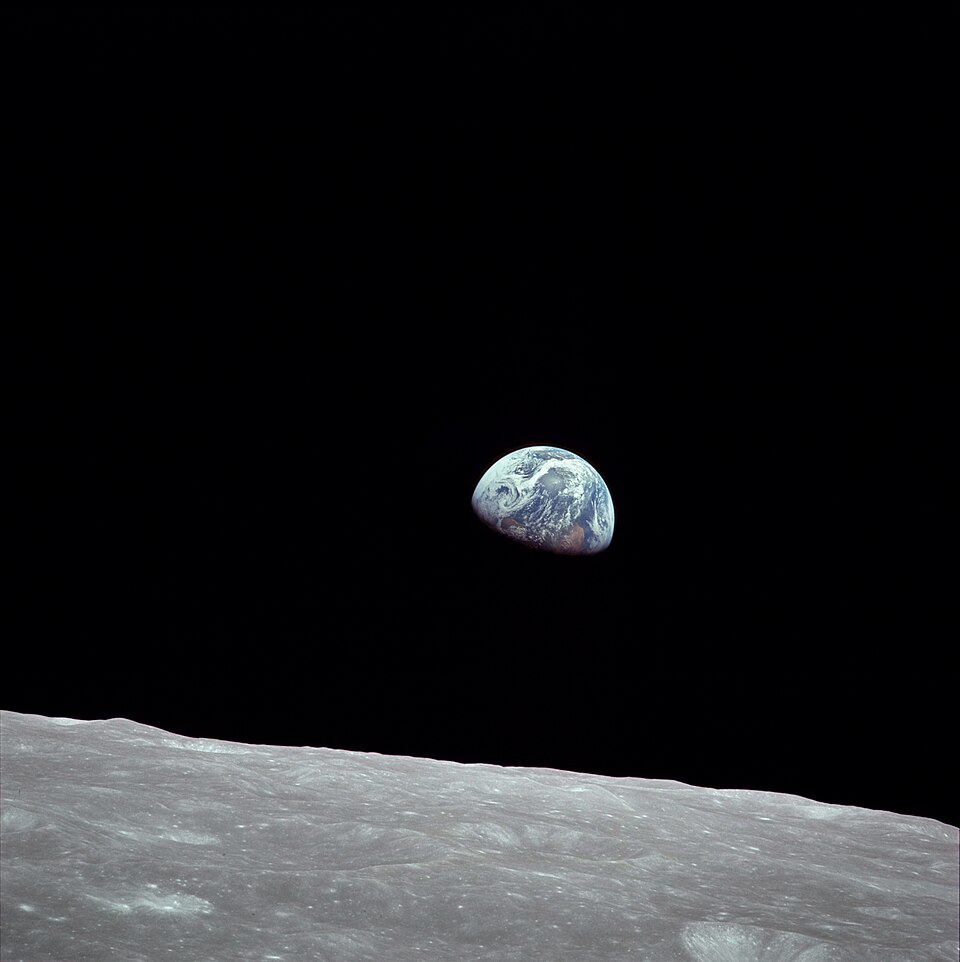
\includegraphics[width=0.85\linewidth]{images/book1/g6-earthrise.jpg}
\end{minipage}\hfill
\begin{minipage}[c]{0.5\linewidth}
{\small \emph{شروق الأرض}: الأرض فوق أفق القمر،
كما صُوّرت من أبولو~8 في مدار حول القمر، 24~ديسمبر~1968.
(الصورة: NASA، بيل أندرز.)}

\medskip
{\small انظر إلى الألوان: زرقة المحيطات، ودوامات السحب
البيضاء، وسمرة اليابسة. وحولها كلها سواد الفضاء؛ وفي
المستوى الأمامي، أرض القمر الرمادية الميتة، بلا ماء وبلا
هواء.}
\end{minipage}
% ledger: nasa:earthrise
\end{omfigure}

الأرض كما تُرى من الفضاء زرقاء في معظمها: \omterm{def:g2:water-on-earth:ocean}{فالمحيط} يغطي نحو سبعة
أعشار سطحها. وتدور فوقها \omterm{def:g4:clouds-rain-snow:cloud}{سحب} بيضاء من قطيرات الماء، ويغطي
جليد أبيض \omterm{def:g3:continents-and-oceans:poles}{القطبين}. واليابسة بنية حيث تكون جافة، وخضراء حيث
تنمو النباتات. والهواء نفسه لا يُرى، لكن \omterm{def:g4:clouds-rain-snow:cloud}{السحب} الطافية فيه
تبين أنه موجود. ومن بين كواكب المجموعة الشمسية كلها، لا تُظهر هذه الألوان
مجتمعة إلا الأرض: الماء السائل، \omterm{def:g4:clouds-rain-snow:cloud}{والسحب}، والنباتات الحية.
% ledger: wss:ocean-cover, nasa:apollo17-earth

\begin{history}[النقطة الزرقاء الباهتة]
\begin{minipage}[c]{0.66\linewidth}
في 14~فبراير~1990، كان المسبار الفضائي فوياجر~1 على بعد نحو 6~مليارات
كيلومتر من الشمس، أبعد من نبتون. وقبل أن يترك
المجموعة الشمسية وراءه، أدار آلة تصويره والتقط صورة
للأرض. وفي الصورة، يبدو كوكبنا ذرة لامعة واحدة، أصغر من
حبة غبار، عالقة في شعاع من ضوء الشمس. وكتب عنها الفلكي كارل ساغان:
«انظر مرة أخرى إلى تلك النقطة. هذا هو هنا. هذا هو بيتنا. هذا
نحن.»
% ledger: nasa:pale-blue-dot
\end{minipage}\hfill
\begin{minipage}[c]{0.3\linewidth}\centering
\begin{tikzpicture}
  \node[inner sep=0] (img) {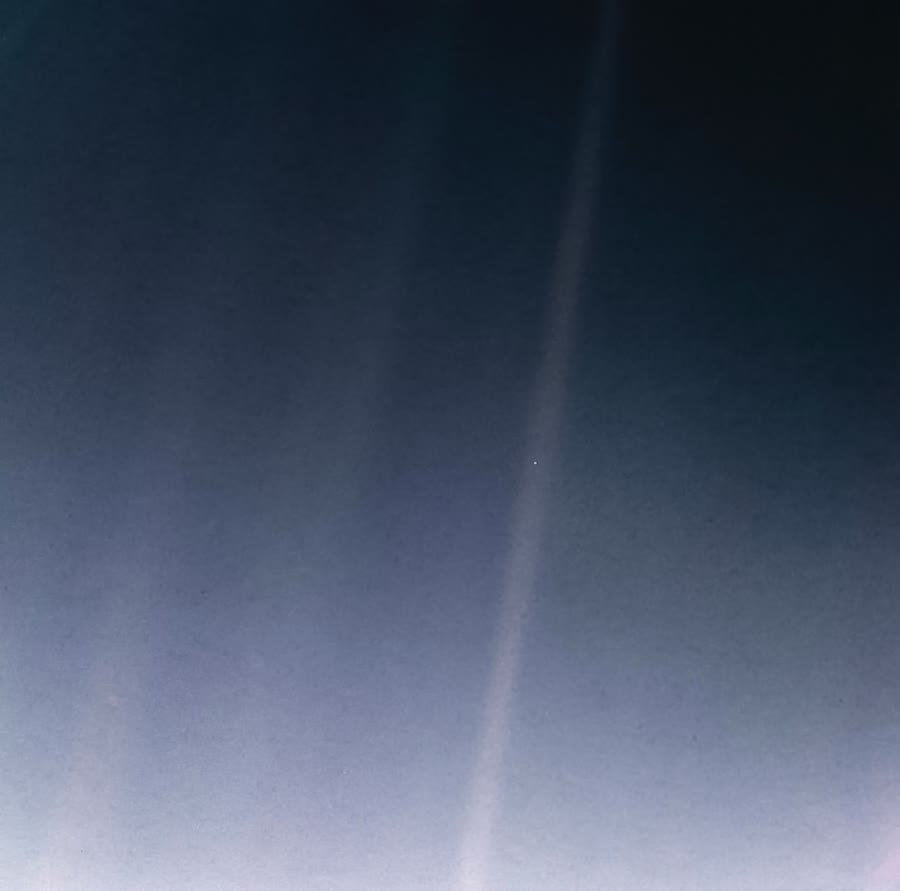
\includegraphics[width=\linewidth]{images/book1/g6-pale-blue-dot.jpg}};
  \draw[yellow!80!orange, thick] ($(img.south west)!0.594!(img.south east) + (0,{0.476*\linewidth})$) circle (6pt);
\end{tikzpicture}\\[2pt]
{\footnotesize الأرض (داخل الدائرة) كما رآها فوياجر~1، عام 1990. (الصورة:
NASA/JPL-Caltech، ملك عام.)}
% ledger: nasa:pale-blue-dot
\end{minipage}
\end{history}

\section{تمارين}

\begin{exercise}[$\star$]\label{exo:g6:earth-a-planet:1}
اذكر كواكب المجموعة الشمسية الثمانية بالترتيب، من الأقرب إلى
الشمس إلى الأبعد. ضع خطًا تحت \omterm{def:g6:earth-a-planet:planet-types}{الكواكب الصخرية}.
\end{exercise}

\begin{exercise}[$\star$]\label{exo:g6:earth-a-planet:2}
انقل وأكمل: «\omterm{def:g6:earth-a-planet:planet-types}{الكوكب الصخري} صغير و\ldots، وله سطح
\ldots{} \omterm{def:g6:earth-a-planet:planet-types}{والكوكب العملاق} كبير جدًا، قليل \ldots، مصنوع في معظمه من
\ldots{} و\ldots{}»
\end{exercise}

\begin{exercise}[$\star$]\label{exo:g6:earth-a-planet:3}
مستعينًا بجدول هذا الفصل، أي كوكب قطره أقرب إلى
قطر الأرض؟ وأي كوكب أكبر الكواكب؟ وأيها أصغرها؟
\end{exercise}

\begin{exercise}[$\star$]\label{exo:g6:earth-a-planet:4}
صواب أم خطأ؟ صحّح الجمل الخاطئة.
(أ) الزهرة مغطاة بالمحيطات.
(ب) المريخ أبرد من الأرض.
(ج) \omterm{def:g6:earth-a-planet:planet-types}{الكواكب العملاقة} هي الكواكب الأربعة الأقرب إلى الشمس.
(د) زحل أقل كثافة من الماء.
\end{exercise}

\begin{exercise}[$\star\star$]\label{exo:g6:earth-a-planet:5}
قطر عطارد 4\,879~كيلومترًا، وقطر الأرض
12\,756~كيلومترًا. احسب قطر عطارد نسبةً مئوية من قطر
الأرض، مقرّبة إلى أقرب عدد صحيح.
% ledger: planet:Mercury.diameter, planet:Earth.diameter (planets.py: 38.2 %)
\end{exercise}

\begin{exercise}[$\star\star$]\label{exo:g6:earth-a-planet:6}
كم أرضًا، جنبًا إلى جنب، تتسع على طول قطر زحل
(120\,536~كيلومترًا)؟ قرّب إلى أقرب عدد صحيح. وهل زحل \omterm{def:g6:earth-a-planet:planet-types}{كوكب صخري}
أم \omterm{def:g6:earth-a-planet:planet-types}{كوكب عملاق}؟
% ledger: planet:Saturn.diameter, planet:Earth.diameter
\end{exercise}

\begin{exercise}[$\star\star$]\label{exo:g6:earth-a-planet:7}
وجد الفلكيون كواكب حول نجوم أخرى. فالكوكب~A كثافته
1.1~غرام لكل سنتيمتر مكعب، وهو أعرض من الأرض 9~مرات.
والكوكب~B كثافته 5.0~غرامات لكل سنتيمتر مكعب، وهو أصغر
قليلًا من الأرض. أيهما \omterm{def:g6:earth-a-planet:planet-types}{كوكب صخري} وأيهما \omterm{def:g6:earth-a-planet:planet-types}{كوكب
عملاق}؟ اشرح.
\end{exercise}

\begin{exercise}[$\star\star$]\label{exo:g6:earth-a-planet:8}
مستعينًا بمخطط درجات حرارة الكواكب: (أ) كم درجة
تزيد حرارة الزهرة على حرارة الأرض؟ (ب) كم درجة يزيد المريخ برودةً على
الأرض؟
% ledger: planet:Venus.Tmean, planet:Earth.Tmean, planet:Mars.Tmean
\end{exercise}

\begin{exercise}[$\star\star$]\label{exo:g6:earth-a-planet:9}
عطارد أقرب الكواكب إلى الشمس، لكن الزهرة أحرها. اشرح
السبب.
\end{exercise}

\begin{exercise}[$\star\star$]\label{exo:g6:earth-a-planet:10}
تقع الأرض على بعد 150~مليون كيلومتر من الشمس، والمريخ على بعد 228~مليون
كيلومتر. بكم مليون كيلومتر يزيد بعد المريخ عن الشمس؟ وبأي
نسبة مئوية يزيد بعد المريخ على بعد الأرض (قرّب إلى
أقرب عدد صحيح)؟
% ledger: planet:Earth.dist, planet:Mars.dist
\end{exercise}

\begin{exercise}[$\star\star\star$]\label{exo:g6:earth-a-planet:11}
يقول صديق: «المريخ كان دائمًا \omterm{def:g5:weather-and-climate:desert}{صحراء} جافة؛ ولم يكن فيه أبدًا
أي ماء.» مستعينًا بهذا الفصل، أجبه: ماذا كان في المريخ
قبل مليارات السنين، وأين ماؤه اليوم، ولماذا لا يستطيع الماء السائل
أن يدوم على سطحه الآن؟
\end{exercise}

\begin{exercise}[$\star\star\star$]\label{exo:g6:earth-a-planet:12}
تسمى الزهرة أحيانًا توأم الأرض. فقطرها 95~\% من قطر
الأرض، وشدة الجاذبية على سطحها 8.9 على سلم تكون فيه شدة
جاذبية الأرض 9.8. (أ) احسب شدة جاذبية الزهرة نسبةً مئوية من شدة جاذبية
الأرض،
مقرّبة إلى أقرب عدد صحيح. (ب) اذكر أمرين تشبه فيهما الزهرة
توأمًا للأرض، وأمرين لا تشبهها فيهما.
% ledger: planet:Venus.gravity, planet:Earth.gravity, planet:Venus.diameter
\end{exercise}

\section{مسألة: بطاقات بريدية من ثلاثة كواكب}

\begin{problem}[{مسألة نهاية الأسبوع --- ثلاث بطاقات بريدية من الفضاء، وكم يضغط
هواء الزهرة على أرضها}]
\label{pb:g6:earth-a-planet:1}
% ledger: planet:Venus.dist, planet:Venus.diameter, planet:Venus.density, planet:Venus.Tmean, planet:Venus.psurf, planet:Earth.dist, planet:Earth.diameter, planet:Earth.density, planet:Earth.Tmean, planet:Earth.psurf, planet:Mars.dist, planet:Mars.diameter, planet:Mars.density, planet:Mars.Tmean, planet:Mars.psurf, nasa:venus-clouds, nasa:mars-water
ترسل ثلاثة مسابير آلية كل منها بطاقة بريدية، كُتبت على
ظهرها بضعة أعداد.

\begin{center}
\small
\begin{tabular}{>{\raggedright\arraybackslash}p{0.29\linewidth}>{\raggedright\arraybackslash}p{0.29\linewidth}>{\raggedright\arraybackslash}p{0.29\linewidth}}
\hline
\textbf{من الزهرة} & \textbf{من الأرض} & \textbf{من المريخ}\\
\hline
البعد عن الشمس: 108~مليون~كيلومتر. & البعد عن الشمس:
150~مليون~كيلومتر. & البعد عن الشمس: 228~مليون~كيلومتر.\\
القطر: 12\,104~كيلومترًا. & القطر: 12\,756~كيلومترًا. & القطر: 6\,792~كيلومترًا.\\
الكثافة: \babelsublr{5.2~g/cm$^3$}. & الكثافة: \babelsublr{5.5~g/cm$^3$}. & الكثافة: \babelsublr{3.9~g/cm$^3$}.\\
متوسط درجة الحرارة: \babelsublr{464~$^\circ$C}. & متوسط درجة الحرارة: \babelsublr{15~$^\circ$C}. &
متوسط درجة الحرارة: \babelsublr{$-65$~$^\circ$C}.\\
يضغط الهواء على الأرض بقوة 92~بارًا. \omterm{def:g4:clouds-rain-snow:cloud}{سحب} كثيفة من الحمض. &
يضغط الهواء على الأرض ببار واحد. محيطات \omterm{def:g4:clouds-rain-snow:cloud}{وسحب}. &
يضغط الهواء على الأرض بقوة 0.01~بار. جليد عند \omterm{def:g3:continents-and-oceans:poles}{القطبين}.\\
\hline
\end{tabular}
\end{center}

\medskip
\noindent\textbf{الجزء الأول --- مقارنة الكواكب.}
\begin{enumerate}
  \item رتّب الكواكب الثلاثة بحسب بعدها عن الشمس.
  \item بكم مليون كيلومتر تقرب الزهرة من الشمس أكثر من
        الأرض؟ وبكم مليون كيلومتر يبعد المريخ أكثر منها؟
  \item احسب قطر المريخ نسبةً مئوية من قطر الأرض،
        مقرّبة إلى أقرب عدد صحيح. هل المريخ نحو ربع عرض الأرض، أم
        نصفه، أم ثلاثة أرباعه؟
  \item هل الكواكب الثلاثة \omterm{def:g6:earth-a-planet:planet-types}{كواكب صخرية} أم \omterm{def:g6:earth-a-planet:planet-types}{كواكب عملاقة}؟ وأي الأعداد
        على البطاقات تخبرك بذلك؟
\end{enumerate}

\medskip
\noindent\textbf{الجزء الثاني --- الهواء.}
\begin{enumerate}[resume]
  \item على أي كوكب يكون الهواء أسمك؟ وعلى أيها يكون
        أرقّ؟
  \item كم مرة يقل ضغط هواء المريخ على أرضه عن ضغط
        هواء الأرض على أرضنا؟
  \item الزهرة أقرب إلى الشمس من الأرض، لكن ذلك وحده لا
        يفسر درجة حرارة تبلغ \babelsublr{464~$^\circ$C}. فماذا يفعل هواء الزهرة
        بحرارة الشمس؟
  \item كم مرة يزيد ضغط الهواء على أرض الزهرة على ضغطه على
        أرض الأرض؟ ولماذا يجب أن تكون جدران المسبار الذي يهبط على الزهرة متينة جدًا؟
\end{enumerate}

\medskip
\noindent\textbf{الجزء الثالث --- الماء والحياة.}
\begin{enumerate}[resume]
  \item عند سطح الأرض، يتجمد الماء عند \babelsublr{0~$^\circ$C} ويغلي عند
        \babelsublr{100~$^\circ$C}. مستعينًا بمتوسطات درجات الحرارة، اشرح لماذا يكون الماء
        سائلًا على الأرض.
  \item ماذا يحدث لكأس ماء موضوعة على أرض
        الزهرة؟ وعلى أرض المريخ؟
  \item كانت في المريخ \omterm{def:g1:landscapes-around-us:water}{أنهار} \omterm{def:g1:landscapes-around-us:water}{وبحيرات} قبل مليارات السنين. فماذا يخبرنا
        ذلك عن \omterm{def:g5:weather-and-climate:climate}{مناخ} المريخ قديمًا، مقارنةً باليوم؟
  \item اكتب ظهر بطاقة الأرض البريدية: في بضع جمل، اذكر
        أربعة أسباب تجعل الحياة ممكنة على الأرض.
\end{enumerate}
\end{problem}
